\documentclass[11pt]{article}

\usepackage[margin=1in]{geometry}
\usepackage{amsmath,amssymb,amsfonts,amsthm}
\usepackage{bm}
\usepackage{hyperref}
\usepackage{graphicx}

\newtheorem{theorem}{Theorem}
\newtheorem{lemma}{Lemma}
\newtheorem{corollary}{Corollary}
\newtheorem{proposition}{Proposition}
\newtheorem{remark}{Remark}
\newtheorem{definition}{Definition}
\newtheorem{assumption}{Assumption}

\newcounter{algorithm}
\newenvironment{paperalgorithm}[1]{%
  \refstepcounter{algorithm}%
  \par\medskip
  \noindent\hrule
  \vspace{0.45em}
  \noindent\textbf{Algorithm~\thealgorithm. #1}\par\vspace{0.35em}
}{%
  \vspace{0.35em}
  \noindent\hrule
  \par\medskip
}

\title{Notes on Laplacian-Coupled Networks of\\
NDR Memristive FitzHugh--Nagumo Motifs}
\author{}
\date{}

\begin{document}

\maketitle
\tableofcontents


\section{What these notes are about}

These are working notes on a concrete physical question: what happens
when you take $N$ active memristive neuron circuits and wire their
exposed voltage nodes together through an ordinary resistor network?
The circuits are the NDR memristive FitzHugh--Nagumo motifs of Pei et
al.~\cite{pei2025}. One reason this question matters is that it has become clear in
our work that a single memristor, one with a unique fixed point,
does not spontaneously develop multiple fixed points when you couple it
to others of the same kind --- roughly, $1^M = 1$. So if you want
associative memory, you need the building blocks to already be bistable
on their own, before coupling enters the picture. That is why we focus
on NDR motifs: each one is natively bistable and acts as a one-bit
memory element. The coupling then has a chance to do something
interesting.

The short physical answer is that the resistor network acts as a
diffusive coupling, with a strength set by the ratio of the inter-node
conductance to the nodal capacitance. The longer answer, which these
notes work out carefully, is that any stable resting state of an
isolated motif survives that coupling and stays stable, as long as the
coupling is not too strong. The argument runs from the device level
upward: we characterise the NDR memristor, assemble the FitzHugh--Nagumo
motif from it, and apply Kirchhoff's laws to get the equations of motion
for the whole network. The result is a smooth perturbation of $N$
non-interacting copies of the same two-dimensional oscillator. Two
standard tools --- the Implicit Function Theorem and the continuity of
eigenvalues --- then do the heavy lifting.

The same framework also covers the case where small voltage sources
sit in series with the coupling resistors. Circuit-wise, these
model synaptic reversal potentials; in the dimensionless FN equations
they appear as a node-wise bias that shifts the fixed points without
touching their stability.

\subsection*{The logical skeleton}

It is worth spelling out the structure of the argument before diving
into circuit algebra, because otherwise it is easy to get lost in the
bookkeeping.

When the coupling resistors are absent --- or equivalently, when their
resistance is infinite --- the $N$ motifs do not interact. Each motif
$i$ obeys its own two-dimensional ODE,
\begin{equation}
  \dot X_i = G(X_i),
  \qquad X_i = (x_i, y_i)^T \in \mathbb{R}^2,
  \label{eq:strategy_decoupled}
\end{equation}
and the joint state $X = (X_1,\ldots,X_N)$ is just the direct product
$\dot X = F_0(X) := (G(X_1),\ldots,G(X_N))$.

Before saying anything about stability, though, we need to be clear
about which dynamical regime we are in, because the FitzHugh--Nagumo
system has two qualitatively different behaviours and only one of them
is relevant here.

In the \emph{oscillatory regime}, the single fixed point sits on the
middle, unstable branch of the cubic voltage nullcline, where the
differential conductance is positive and the Jacobian has a positive
trace. The fixed point is an unstable spiral, and a stable limit cycle
lives around it. In plain language, the motif oscillates indefinitely
and never settles anywhere. There is nothing to perturb stably, so the
programme of these notes simply does not apply.

In the \emph{bistable regime} --- the one we stay in throughout --- the
linear recovery nullcline cuts the cubic voltage nullcline at three
distinct points. The two outer intersections, $p_1$ on the left branch
and $p_3$ on the right, lie where $|x_j| > 1$, in the NDR region where
the differential conductance is negative. There, by the Routh--Hurwitz
criterion, both $p_1$ and $p_3$ are linearly stable fixed points; small
perturbations decay exponentially. The middle intersection $p_2$, with
$|x_2| < 1$, is always a saddle: it is unstable and acts only as the
boundary between the two basins of attraction. The motif does not
oscillate in this regime --- the limit cycle was destroyed as the
parameters moved into the bistable window.

The two regimes are separated by bifurcations in the $(a, b, z)$
parameter space. As the stimulus $z$ increases past a saddle-node
value, the outer fixed points collide and annihilate, the bistable
window closes, and the system transitions to monostable oscillation.
The Pei et al.\ device is designed to operate in the bistable regime,
where it acts as a two-state memory element rather than a clock.

A fixed point $p_j$ is \emph{Hurwitz} if all eigenvalues of the
Jacobian $DG(p_j)$ have strictly negative real part. In the bistable
regime, $p_1$ and $p_3$ satisfy this. The product system therefore has
$M^N = 3^N$ fixed points in total, of which $2^N$ are Hurwitz --- those
in which every node sits at $p_1$ or $p_3$ --- and the remaining
$3^N - 2^N$ involve at least one saddle and are unstable.

Now we turn on the resistors. We introduce a single overall conductance
scale $\bar{g} = 1/R_0$ and write the conductance Laplacian as
$L_G = \bar{g} L$, where $L$ is a dimensionless graph Laplacian with
entries of order one. The coupling parameter is
\begin{equation}
  \varepsilon = \frac{\bar{g}}{C_0} = \frac{1}{R_0 C_0},
  \label{eq:epsilon_strategy}
\end{equation}
the inverse of the $RC$ time constant of the intermediate network
relative to the nodal capacitance. Weak coupling means $\varepsilon \ll
1$, that is, $R_0 \gg 1/C_0$. Sending $R_0 \to \infty$ recovers the
uncoupled system. The coupled network then takes the form
\begin{equation}
  \dot X = F_0(X) + \varepsilon H(X),
  \label{eq:strategy_coupled}
\end{equation}
a smooth $O(\varepsilon)$ deformation of the product system.

The key property of each Hurwitz fixed point $p_j$ is that
$\det DG(p_j) \neq 0$. This means $\det DF_0(P_\alpha) \neq 0$ for
every product fixed point $P_\alpha$, and the Implicit Function Theorem
guarantees that, for small enough $\varepsilon$, each $P_\alpha$
deforms continuously into a nearby fixed point $P_\alpha(\varepsilon)$
of the coupled system. Eigenvalue continuity then ensures that, since
all eigenvalues of $DF_0(P_\alpha)$ started in the open left half-plane
with some spectral gap $\gamma_\alpha > 0$, they cannot cross the
imaginary axis for small $\varepsilon$. Taking the minimum over the
finite set of multi-indices gives a uniform threshold $\varepsilon_* > 0$
valid simultaneously for all $2^N$ Hurwitz product fixed points.

The upshot: \emph{work in the bistable regime, where each isolated motif
has two stable fixed points and no limit cycle; turn on weak coupling;
all $2^N$ Hurwitz fixed points survive and remain stable}, as long as
$\varepsilon = 1/(R_0 C_0)$ is small enough.


\section{The NDR memristor and the FitzHugh--Nagumo motif}
\label{sec:motif}


\subsection{The NDR memristor}

An active negative-differential-resistance (NDR) device is a
two-terminal element that, over some voltage range, delivers more
current as the voltage is \emph{reduced}. This is obviously impossible
for an ordinary resistor and requires either an internal energy source
or a quantum-mechanical transport mechanism. Writing the terminal
current as $I = \phi(V,\xi)$, where $V$ is the applied voltage and
$\xi$ is a vector of internal state variables, the NDR region is where
\begin{equation}
  g_{\mathrm{diff}}(V,\xi)
  =
  \frac{\partial \phi}{\partial V}(V,\xi) < 0.
  \label{eq:ndr_def}
\end{equation}
The device can then supply incremental power to the surrounding circuit,
which is what makes NDR elements useful for sustaining oscillations: a
negative resistance in a loop with a capacitor compensates dissipation
and allows self-amplification. This is exactly what happens in
voltage-gated sodium channels, where the conductance increases with
depolarisation --- a positive feedback whose mathematical fingerprint is
a folded-cubic $I$--$V$ curve.

The same element is called \emph{memristive} when the internal state
has its own dynamics,
\begin{equation}
  \dot\xi = q(V,\xi),
  \label{eq:memristive_state}
\end{equation}
so the current at any instant depends on the past history of the voltage
through $\xi$~\cite{strukov2008}. Together, \eqref{eq:ndr_def} and
\eqref{eq:memristive_state} define the class of devices we work with.

\begin{definition}[NDR memristive element]
  A two-terminal element is an \emph{NDR memristive element} if its
  terminal current is $I = \phi(V,\xi)$ with $\partial_V\phi < 0$ on
  an open voltage interval, and its internal state obeys
  $\dot\xi = q(V,\xi)$.
\end{definition}

The device used throughout these notes is the NDR memristor of Pei et
al.~\cite{pei2025}, built from an
AlAs/In$_{0.8}$Ga$_{0.2}$As/AlAs quantum-well heterostructure on an
InP substrate. The In$_{0.8}$Ga$_{0.2}$As well is about $3$\,nm thick,
thin enough that electrons are confined into discrete transverse energy
levels. When the applied bias aligns the Fermi level of the emitter
with one of these levels, resonant tunneling through the double AlAs
barrier produces a sharp current peak; increasing the bias detunes the
resonance and the current falls --- this is the NDR region. Atomic
vacancies in the well trap electrons on the upswing and release them on
the downswing, producing the box-type hysteretic $I$--$V$ loop that is
the signature of memristive behaviour.

Because the switching is governed by band structure rather than filament
formation or ion migration, the device is unusually robust:
cycle-to-cycle variation in peak and valley currents is below $0.3\%$,
endurance exceeds $10^{11}$ cycles at room temperature and $10^9$
cycles at $400\,{}^\circ\mathrm{C}$, and the peak-to-valley current
ratio remains above $1.86$ across that entire range~\cite{pei2025}.
In our language, $\xi$ encodes the occupancy of the vacancy trapping
sites, and $\dot\xi = q(V,\xi)$ is slow compared with the oscillation
period, which is why the device shows hysteresis rather than
instantaneous switching. The effective negative resistance in the NDR
region is
\begin{equation}
  R_n = \frac{2\Delta V}{3\Delta I},
  \qquad
  \Delta V = V_p - V_v,\quad \Delta I = I_p - I_v,
  \label{eq:Rn}
\end{equation}
giving $\partial_V\phi \approx -1/|R_n| < 0$ in the NDR region, as
required by \eqref{eq:ndr_def}.

\subsection{The FitzHugh--Nagumo circuit motif}

The biological inspiration is the Hodgkin--Huxley picture of the action
potential~\cite{hodgkin1952}: fast inward Na$^+$ current drives
depolarisation, slower outward K$^+$ current drives repolarisation, and
the interplay between them creates the spike. In the Pei et al.\
circuit~\cite{pei2025}, two NDR memristors $D_1$ and $D_2$ with
different threshold voltages $V_{\mathrm{th},1} < V_{\mathrm{th},2}$
are connected in parallel and placed in series with an inductor $L_1$.
The device $D_1$ with the lower threshold plays the fast Na$^+$-like
role; $D_2$ switches later and provides the slower K$^+$-like
repolarising current. The inductor acts as the inductive memory element
that, together with the negative resistance, sustains the oscillation.
Importantly, the intrinsic quantum-well capacitance of each device
takes the place of the membrane capacitance, so no external capacitor
is needed.

The aggregate $I$--$V$ characteristic of the $D_1 \| D_2 + L_1$
combination is $I_{\mathrm{motif}} = \phi(V,\xi)$, with $\xi =
(\xi_1, \xi_2)$ encoding both NDR element states. The slow
K$^+$-like state $\xi_2$ becomes the recovery variable $y$ in the
FitzHugh--Nagumo equations --- we make that identification explicit in
Section~\ref{sec:fn_equations}. The motif has been shown to reproduce
nine experimentally verified FN neuron behaviours, including phasic
spiking, tonic bursting, spike accommodation, anodal break excitation,
and all-or-nothing firing~\cite{pei2025}.


\section{Circuit equations for the coupled network}
\label{sec:circuit}


\subsection{Network topology and the incidence matrix}

We consider $N$ identical NDR motifs whose exposed nodes are connected
through a passive resistive network (see Fig.~\ref{fig:db}).

\begin{figure}[h]
    \centering
    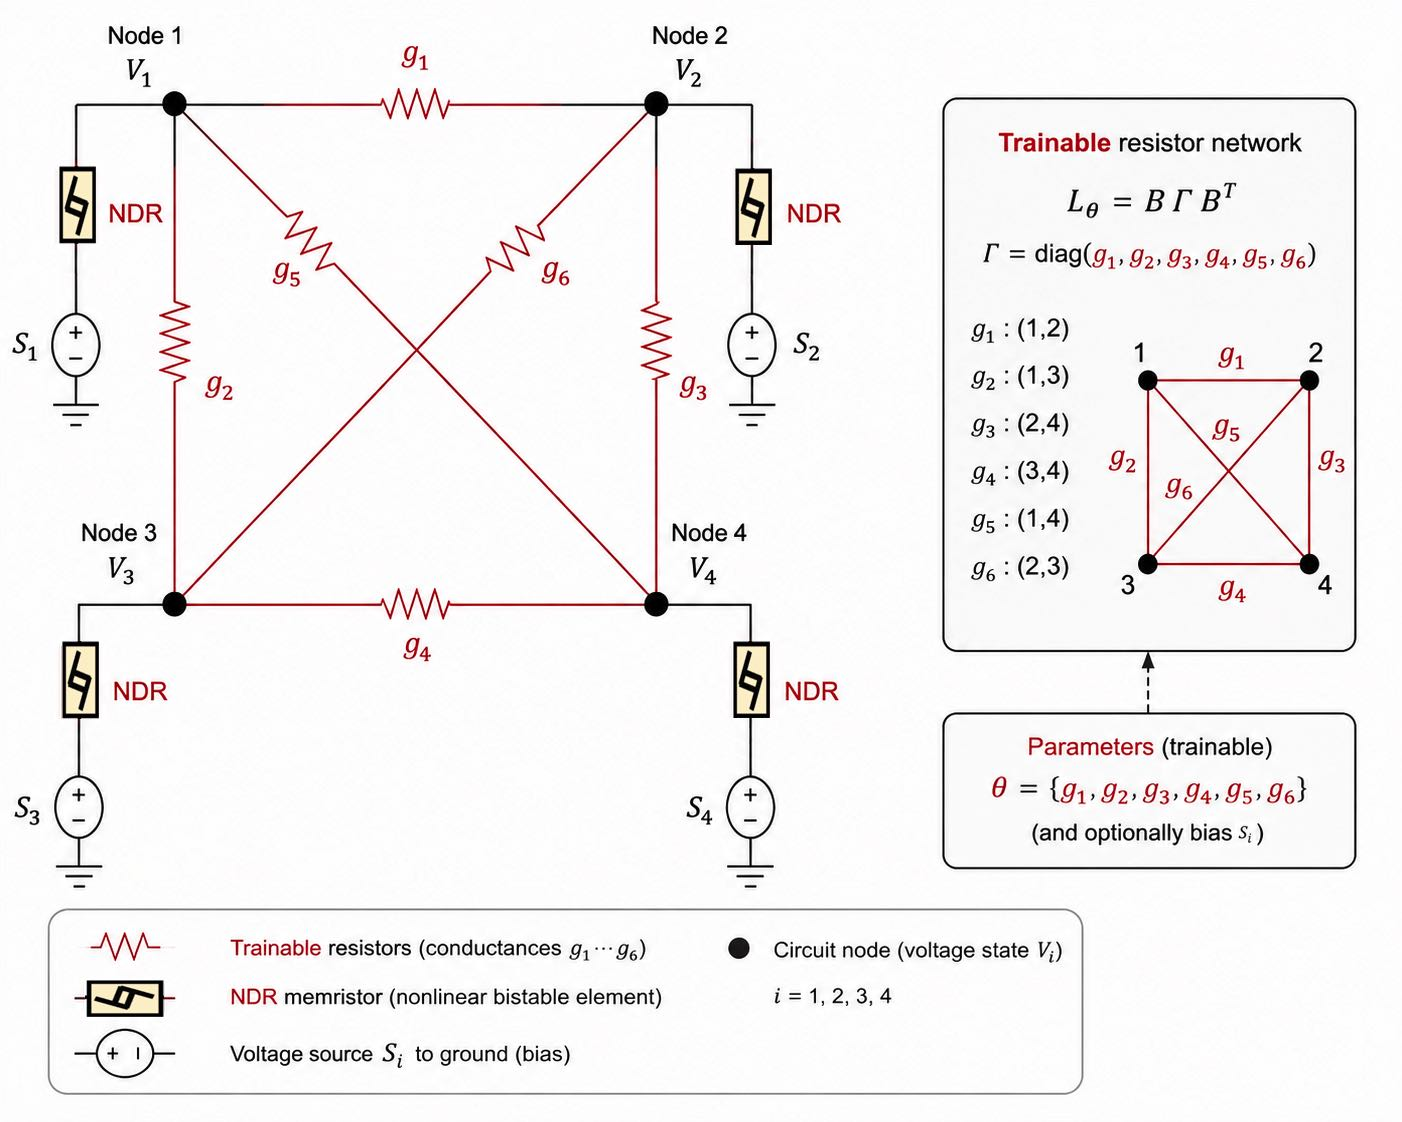
\includegraphics[width=0.5\linewidth]{nodes.jpeg}
    \caption{Schematic of the coupled NDR network. Each node $i$ carries
    an NDR motif $M_i$ and a local bias source $s_i$; the exposed nodes
    are linked by the intermediate resistive network with resistors
    $R_{12}=g_1^{-1}$, $R_{23}=g_6^{-1}$, etc.}
    \label{fig:db}
\end{figure}

Each motif
$i$ exposes one terminal node at voltage $v_i$ and has its other
terminal grounded through the NDR branch, which also contains a fixed
series bias source $s_i$. This bias shifts the effective voltage seen
by the NDR element and will later map onto the applied stimulus $z_i$
in the FitzHugh--Nagumo equations; it can also encode a reversal
potential or a dc offset.

The intermediate network has $E$ edges. We choose an arbitrary
orientation for each edge and encode the topology in the directed
incidence matrix
\begin{equation}
  B \in \mathbb{R}^{N\times E},
  \qquad
  B_{ie}
  =
  \begin{cases}
    +1, & \text{edge } e \text{ enters node } i,\\
    -1, & \text{edge } e \text{ leaves node } i,\\
    0,  & \text{otherwise.}
  \end{cases}
  \label{eq:incidence_def}
\end{equation}
The choice of orientation is arbitrary; the physics does not depend on
it. We collect node voltages, edge currents, and conductances:
\begin{equation}
  v = (v_1,\ldots,v_N)^T,
  \quad
  j = (j_1,\ldots,j_E)^T,
  \quad
  G = \operatorname{diag}(g_1,\ldots,g_E).
\end{equation}

For motif $i$, let $i_i$ be the NDR branch current oriented from the
exposed node toward ground. The voltage the NDR element actually sees
is $m_i = v_i - s_i$, so
\begin{equation}
  i_i = \phi_i(v_i - s_i,\, \xi_i),
  \qquad
  \dot\xi_i = q_i(v_i - s_i,\, \xi_i).
  \label{eq:ndr_current_voltage}
\end{equation}
In vector form,
\begin{equation}
  i = \phi(v - s,\,\xi),
  \qquad
  \dot\xi = q(v - s,\,\xi).
  \label{eq:vector_ndr}
\end{equation}

\subsection{Kirchhoff's laws and the conductance Laplacian}

Ohm's law on each resistive edge gives~\cite{desoer1969}
\begin{equation}
  j = G\,B^T v.
  \label{eq:edge_current_from_node_voltage}
\end{equation}
Kirchhoff's current law says the net current flowing back into node $i$
from the network is $-(Bj)_i$. Substituting Ohm's law,
\begin{equation}
  i_{\mathrm{net}} = -B j = -B G B^T v = -L_G v,
  \label{eq:network_current_injection_laplacian}
\end{equation}
where
\begin{equation}
  L_G = B G B^T \in \mathbb{R}^{N\times N}.
  \label{eq:conductance_laplacian}
\end{equation}
This is the \emph{weighted conductance Laplacian} of the intermediate
network~\cite{doyle1984,chung1997}. Its emergence here is not a
modelling choice; it is the unavoidable consequence of combining Ohm's
law and KCL on any resistor network, whatever the topology. Concretely,
the off-diagonal entry $(L_G)_{ij}$ for $i \neq j$ is $-g_{ij}$ (the
conductance of the resistor between nodes $i$ and $j$, or zero if they
are not connected), and the diagonal entry $(L_G)_{ii} = \sum_{j\neq
i}g_{ij}$ is the total conductance attached to node $i$. The matrix is
symmetric and positive semi-definite; it is positive definite when the
graph is connected; and its null space is spanned by the all-ones vector
$\mathbf{1}$, expressing the obvious physical fact that a uniform
voltage shift drives no current because all voltage differences vanish.

Applying KCL at node $i$ gives
\begin{equation}
  C_i \dot v_i = -i_i - (L_G v)_i.
  \label{eq:kcl_scalar_laplacian}
\end{equation}
Substituting \eqref{eq:ndr_current_voltage} and stacking into vectors,
the exact equations of motion are
\begin{equation}
  {C\dot v = -\phi(v - s, \xi) - L_G v,}
  \label{eq:full_network_voltage}
\end{equation}
\begin{equation}
  {\dot\xi = q(v - s, \xi),}
  \label{eq:full_network_internal}
\end{equation}
with $C = \operatorname{diag}(C_1,\ldots,C_N)$. These two equations,
derived from nothing beyond Ohm's law and KCL, are the exact equations
of motion for any network of NDR memristive elements connected by
resistors.

Writing $L_G = \bar{g}\,L$ and assuming identical nodal capacitances
$C_i = C_0$, the voltage equation becomes
\begin{equation}
  \dot v = -\frac{1}{C_0}\phi(v - s, \xi) - \varepsilon L v,
  \qquad
  \varepsilon = \frac{\bar{g}}{C_0}.
  \label{eq:normalized_voltage_eps}
\end{equation}
The dimensionless coupling strength $\varepsilon$ is simply the ratio
of the inter-node conductance scale to the effective nodal capacitance.


\section{The FitzHugh--Nagumo equations and their NDR realisation}
\label{sec:fn_equations}


\subsection{The FitzHugh--Nagumo equations}

The FitzHugh--Nagumo (FN) equations are the canonical two-dimensional
reduction of the Hodgkin--Huxley model~\cite{hodgkin1952}, introduced
independently by FitzHugh~\cite{fitzhugh1961} and by Nagumo, Arimoto,
and Yoshizawa~\cite{nagumo1962}. The key simplification is geometric:
keep the fast voltage variable $x$ with its folded-cubic nullcline and a
slow recovery variable $y$ with a linear nullcline, and everything
else follows. The system is
\begin{equation}
  \dot{x} = x - \frac{x^3}{3} - y + z,
  \qquad
  \dot{y} = \frac{1}{\tau}(x + a - by),
  \label{eq:fn_standard}
\end{equation}
where $z$ is the applied stimulus and $\tau$, $a$, $b$ are
dimensionless parameters. The cubic term is what gives the voltage
nullcline its N-shape, which is responsible for bistability and, when
the fixed point lands on the unstable middle branch, for the limit-cycle
oscillations that model repetitive spiking~\cite{izhikevich2007}.

\subsection{Identifying $\phi$ and $\xi$ with FN variables}

The $I$--$V$ characteristic of the Pei et al.\ motif has exactly the
folded-cubic form the FN model needs (Fig.~\ref{fig:pei}).

\begin{figure}[h]
    \centering
    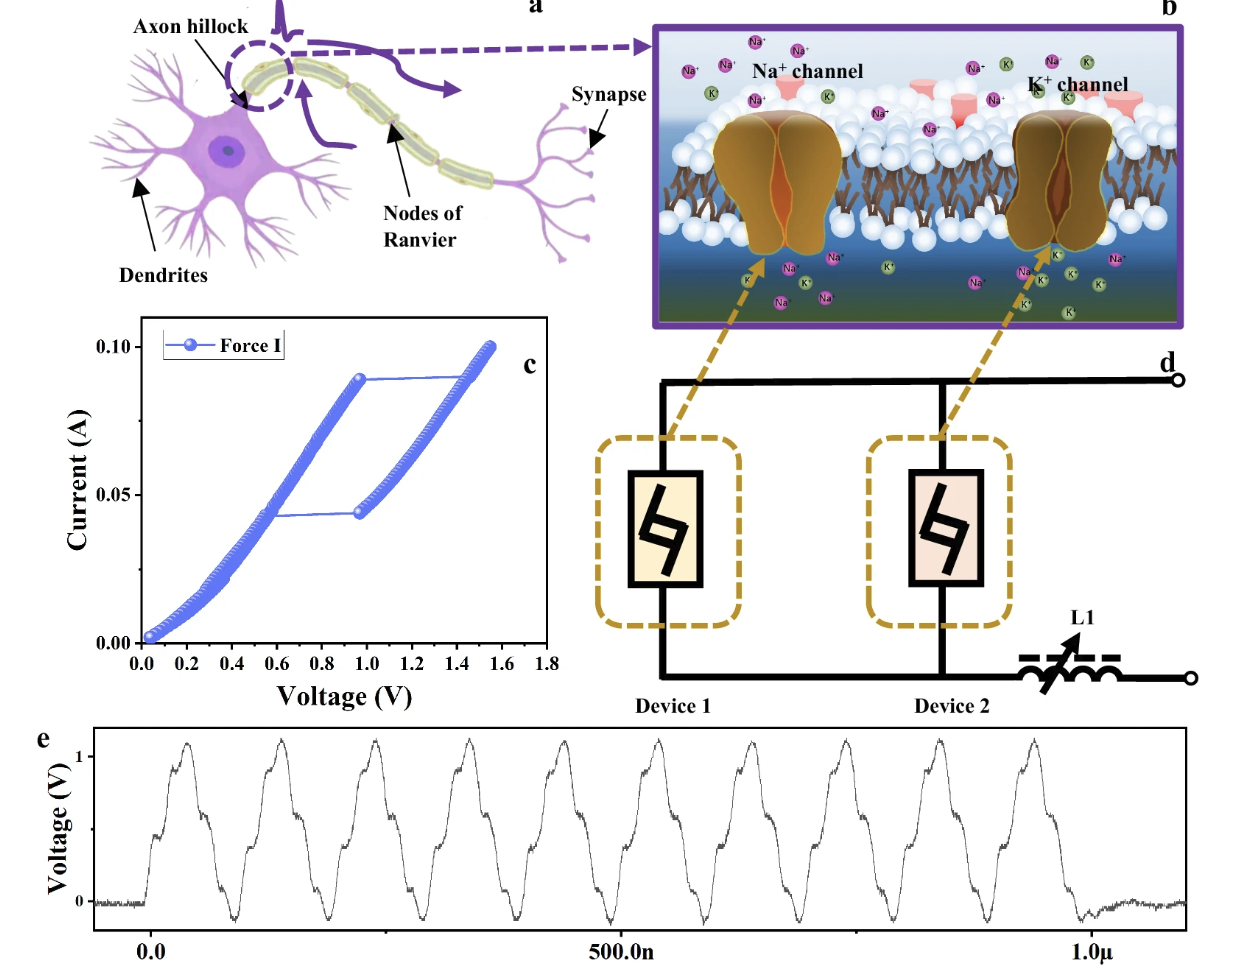
\includegraphics[width=0.5\linewidth]{NDR.png}
    \caption{The $I$--$V$ characteristic of the two-NDR-memristor motif
    (reproduced from \cite{pei2025}), showing the N-shaped negative
    differential resistance region and the box-type hysteresis loop.}
    \label{fig:pei}
\end{figure}

Let $x(t)$
be the dimensionless voltage variable and $y(t)$ the dimensionless
recovery variable. The internal state reduces to $\xi = y$, and the
device functions take the specific forms
\begin{equation}
  \phi(v - s, y)
  \;\longleftrightarrow\;
  -c\!\left(z + x - \frac{x^3}{3} - y\right),
  \qquad
  q(v - s, y)
  \;\longleftrightarrow\;
  \frac{1}{c}(x - a - by),
  \label{eq:fn_identification}
\end{equation}
where $z = s/V_{\mathrm{scale}}$ and $c > 0$ is the time-scale ratio.
The minus sign in the first identification comes from the sign
convention in \eqref{eq:kcl_scalar_laplacian}: the NDR branch current
\emph{leaves} the node, so the current charging the capacitor is
$-\phi_i$. With this identification, the isolated-motif equations
become
\begin{align}
  \dot{x}
  &=
  c\!\left(z + x - \frac{x^3}{3} - y\right),
  \label{eq:fn_x}\\
  \dot{y}
  &=
  \frac{1}{c}(x - a - by).
  \label{eq:fn_y}
\end{align}
We collect the right-hand side into the vector field
\begin{equation}
  G(x,y)
  :=
  \begin{pmatrix}
    c\!\left(z + x - \dfrac{x^3}{3} - y\right)\\[6pt]
    \dfrac{1}{c}(x - a - by)
  \end{pmatrix},
  \label{eq:single_motif}
\end{equation}
so the isolated motif satisfies $(\dot x, \dot y)^T = G(x,y)$.

The time-scale separation is transparent here. The fast equation scales
with $c$; the slow equation runs on time scale $c$, which is long when
$c \gg 1$. In the Pei et al.\ circuit, this separation arises because
$D_1$ switches fast (Na$^+$-like) and $D_2$ switches on a longer time
scale set by its higher threshold voltage, with $L_1$ controlling the
oscillation frequency~\cite{pei2025}.

\subsection{The coupled FN network in dimensionless form}

Substituting the identification \eqref{eq:fn_identification} into
\eqref{eq:normalized_voltage_eps}, the coupled network reads
\begin{align}
  \dot{x}_i
  &=
  c\!\left(z_i + x_i - \frac{x_i^3}{3} - y_i\right)
  -
  \varepsilon\,(Lx)_i,
  \label{eq:coupled_x}\\
  \dot{y}_i
  &=
  \frac{1}{c}(x_i - a - by_i).
  \label{eq:coupled_y}
\end{align}
In vector form,
\begin{align}
  \dot{x}
  &=
  c\!\left(z + x - \tfrac{1}{3}x^{\circ 3} - y\right)
  -
  \varepsilon\,Lx,
  \label{eq:eps_x}\\
  \dot{y}
  &=
  \frac{1}{c}(x - a\mathbf{1} - by).
  \label{eq:eps_y}
\end{align}
Notice that coupling appears only in the voltage equation. This is
physically correct: the resistors link the exposed voltage nodes and
cannot directly drive the recovery variable $y_i$, which is internal
to each motif. Setting $X_i = (x_i, y_i)^T$ and $X =
(X_1,\ldots,X_N)$, the system takes the abstract form
\begin{equation}
  \dot X = \mathcal{F}(X,\varepsilon) = F_0(X) + \varepsilon H(X),
  \label{eq:abstract}
\end{equation}
where $F_0(X) = (G(X_1),\ldots,G(X_N))$ is the product of $N$
uncoupled motif vector fields and $H(X)$ places $-(Lx)_i$ in the
voltage slot of motif $i$ and zero in the recovery slot.

\subsection{Voltage sources in the intermediate network}
\label{sec:voltage_sources}

A natural extension is to place a voltage source $E_e$ in series with
each coupling resistor $R_e$. From a neuroscience perspective, such sources model
synaptic reversal potentials~\cite{dayan2001}: the voltage at which a
synaptic current changes sign, set by the ionic composition of the
junction. They can also model fixed electrochemical offsets or
deliberate bias voltages introduced for circuit control.

With a source $E_e$ on edge $e$, the effective voltage drop across that
resistor is $(B^Tv)_e - E_e$, so Ohm's law becomes $j = G(B^Tv -
e_{\mathrm{src}})$. The nodal injection current becomes
\begin{equation}
  i_{\mathrm{net}} = -Bj = -L_G v + B_E,
  \label{eq:net_current_with_sources}
\end{equation}
where $B_E = BGe_{\mathrm{src}} \in \mathbb{R}^N$ is the
\emph{source-injection vector}. Note that $\mathbf{1}^T B_E = 0$: voltage
sources between nodes inject no net current into the network, which is
just Kirchhoff's current law at the network level. In dimensionless FN
variables, $B_E$ becomes an additive vector $\varepsilon u$ in the
$\dot x$ equation:
\begin{align}
  \dot{x}
  &=
  c\!\left(z + x - \tfrac{1}{3}x^{\circ 3} - y\right)
  -
  \varepsilon Lx
  +
  \varepsilon\, u,
  \label{eq:eps_x_sources}\\
  \dot{y}
  &=
  \frac{1}{c}(x - a\mathbf{1} - by),
  \label{eq:eps_y_sources}
\end{align}
and in abstract form,
\begin{equation}
  \dot X = F_0(X) + \varepsilon H(X) + \varepsilon S(u),
  \label{eq:abstract_sources}
\end{equation}
where $S(u)$ has entries $u_i$ in the voltage slots and zero in the
recovery slots. Since $S(u)$ does not depend on $X$, the Jacobian
$D_X\mathcal{F}$ is the same as in the source-free case. The sources
shift the equilibria without touching their stability type.

\subsubsection*{Perturbative expansion for small sources}

Write $u = \mu\hat{u}$ with $\|\hat{u}\| = 1$ and treat both
$\varepsilon$ and the source amplitude $\mu$ as small. At
$(\varepsilon,\mu) = (0,0)$ the equilibria are the uncoupled product
points $P_\alpha$ defined below. Since $\mathcal{F}$ is $C^1$ and
$D_X F_0(P_\alpha)$ is invertible, the Implicit Function Theorem
applies jointly in $(\varepsilon,\mu)$ and gives a $C^1$ branch
$P_\alpha(\varepsilon,\mu)$ with first-order expansion
\begin{equation}
  P_\alpha(\varepsilon,\mu)
  =
  P_\alpha
  -
  \varepsilon [D_X F_0(P_\alpha)]^{-1} H(P_\alpha)
  -
  \varepsilon\mu [D_X F_0(P_\alpha)]^{-1} S(\hat{u})
  +
  O(\varepsilon^2, \varepsilon\mu^2).
  \label{eq:Palpha_full_expansion}
\end{equation}

Several things are worth noting here. There is no $O(\mu)$ term at all:
because $u$ enters multiplied by $\varepsilon$, sources have no effect
on equilibria when the resistors are disconnected, regardless of how
large $u$ is. This is obvious physically --- voltage sources in an open
circuit carry no current and do nothing. The leading effect of sources
on equilibria is at order $\varepsilon\mu$. At this order the coupling
correction and the source correction are additive. And because $S(u)$
is independent of $X$, the Jacobian at the perturbed equilibrium is the
same as without sources: the equilibria shift but their stability type
is unchanged.

The resolvent $[DG(p_j)]^{-1}$ has a closed form at equilibrium
$p_j = (x_j,y_j)$:
\begin{equation}
  [DG(p_j)]^{-1}
  =
  \frac{1}{1-b+bx_j^2}
  \begin{pmatrix}
    -b/c & c \\
    -1/c & c(1-x_j^2)
  \end{pmatrix}.
  \label{eq:Aj_inv}
\end{equation}
The voltage and recovery shifts at node $i$ due to a source $E_e$ on
edge $e = (i,j)$ are, to leading order in $\varepsilon\mu$,
\begin{equation}
  \Delta x_{\alpha_i}
  \approx
  \frac{\varepsilon\mu\, g_e\, u_e\, b/c}{1 - b + bx_{\alpha_i}^2},
  \qquad
  \Delta y_{\alpha_i}
  \approx
  \frac{\varepsilon\mu\, g_e\, u_e/c}{1 - b + bx_{\alpha_i}^2},
  \label{eq:shifts}
\end{equation}
both of which vanish as $\varepsilon \to 0$ or $\mu \to 0$, and both of
which are well defined whenever $\det DG(p_{\alpha_i}) \neq 0$.


\section{Equilibria and nullclines of the isolated motif}
\label{sec:equilibria}


The equilibria of \eqref{eq:fn_x}--\eqref{eq:fn_y} are where both
time derivatives vanish. Setting $\dot x = 0$ gives the \emph{voltage
nullcline},
\begin{equation}
  y_* = z + x_* - \frac{x_*^3}{3},
  \label{eq:vnull}
\end{equation}
and setting $\dot y = 0$ gives the \emph{recovery nullcline},
\begin{equation}
  y_* = \frac{x_* - a}{b}.
  \label{eq:rnull}
\end{equation}
Eliminating $y_*$ gives the cubic
\begin{equation}
  -\frac{x_*^3}{3}
  +
  \left(1 - \frac{1}{b}\right)x_*
  +
  \left(z + \frac{a}{b}\right)
  = 0.
  \label{eq:cubic_std}
\end{equation}
Three distinct real roots --- hence three equilibria $p_j = (x_j, y_j)$
with $x_1 < x_2 < x_3$ --- occur when the slope $1/b$ of the recovery
line falls between the local maximum and minimum slopes of the cubic and
the stimulus $z$ is in the bistable window.

The Jacobian at any point $(x,y)$ is
\begin{equation}
  DG(x,y)
  =
  \begin{pmatrix}
    c(1-x^2) & -c \\
    1/c & -b/c
  \end{pmatrix}.
  \label{eq:jacobian}
\end{equation}
At equilibrium $p_j = (x_j,y_j)$,
\begin{align}
  \operatorname{tr} DG(p_j)
  &= c(1-x_j^2) - \frac{b}{c},
  \label{eq:trace}\\
  \det DG(p_j)
  &= 1 - b + bx_j^2.
  \label{eq:det}
\end{align}
The Routh--Hurwitz criterion for a $2\times 2$ matrix reduces to two
conditions: trace negative and determinant positive. So $p_j$ is Hurwitz
if and only if
\begin{equation}
  c(1-x_j^2) - \frac{b}{c} < 0
  \quad\text{and}\quad
  1 - b + bx_j^2 > 0.
  \label{eq:hurwitz_conds}
\end{equation}
The first condition is automatically satisfied whenever $|x_j| > 1$,
i.e.\ whenever the equilibrium is on the outer branches of the cubic
where the NDR is active. The middle equilibrium, when $M = 3$, always
has $\det DG(p_2) < 0$: it is a saddle, always unstable.


\section{Persistence and stability under weak coupling}
\label{sec:general}


Here is the analytical argument that the resting states survive
coupling. We state it for a general smooth family of ODEs parameterised
by a small coupling constant, because the same machinery will be reused
twice --- once for coupling alone and once for the joint
coupling-plus-sources problem.

Consider
\begin{equation}
  \dot X = \mathcal{F}(X,\varepsilon),
  \qquad X \in \mathbb{R}^n,\quad \varepsilon \in \mathbb{R},
  \label{eq:gen_system}
\end{equation}
and suppose $X^*$ is a resting state at $\varepsilon = 0$. The
linearisation there is $\dot\xi = A\xi$ with $A = D_X\mathcal{F}(X^*,0)$.
We call $X^*$ \emph{Hurwitz} if all eigenvalues of $A$ have strictly
negative real part, and \emph{hyperbolic} if no eigenvalue is purely
imaginary.

Hurwitz implies hyperbolic, and it implies $\det A \neq 0$ because zero
is on the imaginary axis and cannot be an eigenvalue of a Hurwitz
matrix. This nonsingularity is the key: it is exactly the condition
needed to apply the Implicit Function Theorem and show that the resting
state moves continuously with $\varepsilon$ rather than disappearing.

\begin{theorem}[Persistence of hyperbolic equilibria]
  \label{thm:general_persistence}
  Let $\mathcal{F}:\mathbb{R}^n\times\mathbb{R}\to\mathbb{R}^n$ be $C^1$.
  Suppose $\mathcal{F}(X^*,0)=0$ and $\det D_X\mathcal{F}(X^*,0)\neq 0$.
  Then there exist an open ball $U\ni X^*$ and $\varepsilon_0>0$ such
  that for each $|\varepsilon|<\varepsilon_0$ there is a unique
  $X^*(\varepsilon)\in U$ with $\mathcal{F}(X^*(\varepsilon),\varepsilon)=0$.
  The map $\varepsilon\mapsto X^*(\varepsilon)$ is $C^1$ and $X^*(0)=X^*$.
\end{theorem}

\begin{proof}
  Apply the Implicit Function Theorem~\cite{rudin1976,lang1993} to
  $\mathcal{F}$ at $(X^*,0)$. The hypothesis is exactly the invertibility
  of the partial Jacobian required by that theorem.
\end{proof}

This is the classical statement that hyperbolic fixed points are
structurally stable~\cite{hirsch2013,wiggins2003}: small smooth
perturbations cannot destroy them. Knowing the continued fixed point
$X^*(\varepsilon)$ exists is only half the story, though. We also need
it to stay stable.

\begin{theorem}[Persistence of Hurwitz stability]
  \label{thm:general_hurwitz}
  Under the hypotheses of Theorem~\ref{thm:general_persistence}, if
  additionally $D_X\mathcal{F}(X^*,0)$ is Hurwitz, then there exists
  $0<\varepsilon_1\leq\varepsilon_0$ such that $X^*(\varepsilon)$ is
  Hurwitz and locally asymptotically stable for all
  $|\varepsilon|<\varepsilon_1$.
\end{theorem}

\begin{proof}
  Let $\gamma = -\max_\lambda\operatorname{Re}(\lambda)|_{\varepsilon=0}>0$
  be the spectral gap. The Jacobian $A(\varepsilon) =
  D_X\mathcal{F}(X^*(\varepsilon),\varepsilon)$ is continuous in
  $\varepsilon$ because $\mathcal{F}$ is $C^1$ and $X^*(\varepsilon)$ is
  $C^1$. Eigenvalues are continuous functions of matrix entries --- they
  are roots of the characteristic polynomial, and polynomial roots
  depend continuously on their coefficients~\cite{horn2013}. So if all
  eigenvalues of $A(0)$ lie strictly in the open left half-plane, they
  cannot jump to the right as $\varepsilon$ is turned on; they must stay
  there for some finite interval. Concretely, there exists
  $\varepsilon_1$ such that all eigenvalues of $A(\varepsilon)$ have
  real part at most $-\gamma/2 < 0$ for $|\varepsilon| < \varepsilon_1$.
  Local asymptotic stability follows from Lyapunov's indirect
  method~\cite{khalil2002} via local expansion near a fixed point.
\end{proof}

It is instructive to also have a proof that does not rely on the
abstract continuity of eigenvalues, but instead makes the geometry more
explicit via the Gershgorin discs.

\begin{proof}[Alternative proof via Gershgorin after Schur scaling]
  Since $A(0)$ is Hurwitz, every eigenvalue lies strictly in the open
  left half-plane. Let $\gamma > 0$ be the spectral gap from the
  imaginary axis. The Gershgorin discs of $A(0)$ need not lie in the
  left half-plane in the original coordinates, but a similarity
  transformation can fix that.

  By the complex Schur decomposition, there exists a unitary $Q$ such
  that $Q^*A(0)Q = T$ is upper triangular with diagonal entries
  $T_{ii} = \lambda_i$, the eigenvalues of $A(0)$, each satisfying
  $\operatorname{Re} T_{ii} \leq -\gamma$. Introduce the diagonal
  scaling
  \begin{equation}
    D_\delta
    =
    \operatorname{diag}(1,\delta,\delta^2,\ldots,\delta^{n-1}),
    \qquad
    0<\delta<1,
  \end{equation}
  and define $T_\delta = D_\delta^{-1} T D_\delta$. This matrix is
  similar to $A(0)$ and has the same eigenvalues. Because $T$ is upper
  triangular, the diagonal entries are unchanged: $(T_\delta)_{ii} =
  T_{ii} = \lambda_i$. For $j > i$, however, the off-diagonal entries
  transform as $(T_\delta)_{ij} = \delta^{j-i} T_{ij}$. By choosing
  $\delta$ small enough, we can make the row sums of off-diagonal
  entries uniformly smaller than $\gamma/2$:
  \begin{equation}
    \sum_{j\neq i}|(T_\delta)_{ij}|
    <
    \frac{\gamma}{2}
    \qquad
    \text{for all } i.
  \end{equation}
  The $i$-th Gershgorin disc of $T_\delta$ is then centred at
  $\lambda_i$ (real part $\leq -\gamma$) with radius less than
  $\gamma/2$, so every point in every disc satisfies
  \begin{equation}
    \operatorname{Re}z \leq -\gamma + \frac{\gamma}{2} = -\frac{\gamma}{2} < 0.
  \end{equation}
  Now define $\widetilde A(\varepsilon) = D_\delta^{-1} Q^* A(\varepsilon) Q
  D_\delta$, which is similar to $A(\varepsilon)$ and hence has the same
  eigenvalues. Since $A(\varepsilon) \to A(0)$ as $\varepsilon \to 0$,
  we have $\widetilde A(\varepsilon) \to T_\delta$. Because the
  Gershgorin discs of $T_\delta$ lie a positive distance from the
  imaginary axis, those of $\widetilde A(\varepsilon)$ also remain in
  the open left half-plane for all sufficiently small $|\varepsilon|$.
  Therefore $A(\varepsilon)$ is Hurwitz for small $\varepsilon$, and
  local asymptotic stability follows from Lyapunov's indirect method.
\end{proof}

Applying these theorems to $N$ uncoupled copies of the same system: the
product system $\dot X = F_0(X)$ has exactly $M^N$ equilibria, one for
each way of assigning one of the $M$ local resting states to each node.
Label them
\begin{equation}
  P_\alpha = (p_{\alpha_1},\ldots,p_{\alpha_N}),
  \qquad \alpha \in \{1,\ldots,M\}^N.
\end{equation}
The Jacobian at $P_\alpha$ is block diagonal,
\begin{equation}
  DF_0(P_\alpha) = \operatorname{diag}(DG(p_{\alpha_1}),\ldots,DG(p_{\alpha_N})),
\end{equation}
with determinant $\prod_i\det DG(p_{\alpha_i})\neq 0$ and spectrum equal
to the union of the individual spectra.

\begin{corollary}[Product equilibria]
  \label{cor:product}
  If $G:\mathbb{R}^m\to\mathbb{R}^m$ is $C^1$ with $M$ distinct
  hyperbolic equilibria, then $\dot X = F_0(X)$ has exactly $M^N$
  hyperbolic product equilibria. Every $P_\alpha$ whose component
  equilibria are all Hurwitz is itself Hurwitz.
\end{corollary}

Applying Theorems~\ref{thm:general_persistence} and
\ref{thm:general_hurwitz} to the perturbed product system: all $M^N$
product equilibria survive and those that were Hurwitz remain Hurwitz,
for $\varepsilon$ small enough.


\section{Equilibria and stability of the coupled network}
\label{sec:main}


We now apply the abstract results directly to the NDR--FN network
\eqref{eq:abstract}.

\begin{assumption}
  \label{ass:hyp}
  The FN parameters $(a,b,c,z)$ are such that the isolated motif has
  $M$ distinct equilibria $p_1,\ldots,p_M$, each hyperbolic. In
  practice, either the motif is monostable ($M=1$, one resting state)
  or bistable ($M=3$, two stable outer resting states separated by a
  saddle).
\end{assumption}

Under this assumption, Corollary~\ref{cor:product} gives $M^N$
hyperbolic product equilibria for the uncoupled network. Their Jacobian
determinant factorises as
\begin{equation}
  \det D_X F_0(P_\alpha)
  =
  \prod_{i=1}^{N}(1 - b + bx_{\alpha_i}^2) \neq 0,
  \label{eq:block_det}
\end{equation}
each factor being $\det DG(p_{\alpha_i})$, nonzero by hyperbolicity.

\begin{theorem}[Persistence and stability for the NDR--FN network]
  \label{thm:main}
  Let Assumption~\ref{ass:hyp} hold. Consider the Laplacian-coupled
  network \eqref{eq:eps_x}--\eqref{eq:eps_y} with coupling strength
  $\varepsilon = \bar{g}/C_0$. For each multi-index
  $\alpha = (\alpha_1,\ldots,\alpha_N)\in\{1,\ldots,M\}^N$, let
  $P_\alpha = (p_{\alpha_1},\ldots,p_{\alpha_N})$ be the corresponding
  product equilibrium of the uncoupled network. Then:

  \begin{enumerate}
    \item[\textup{(i)}] \textup{(Persistence.)}
    For each $\alpha$, there exist $\varepsilon_\alpha>0$ and a
    neighbourhood $U_\alpha$ of $P_\alpha$ such that, for every
    $|\varepsilon|<\varepsilon_\alpha$, the coupled network has a unique
    equilibrium $P_\alpha(\varepsilon)\in U_\alpha$ with
    $P_\alpha(0)=P_\alpha$, depending $C^1$-smoothly on $\varepsilon$.

    \item[\textup{(ii)}] \textup{(Stability.)}
    If $p_{\alpha_1},\ldots,p_{\alpha_N}$ are all Hurwitz, then there
    exists $0<\varepsilon_{\alpha}^{\mathrm{H}}\leq\varepsilon_\alpha$
    such that $P_\alpha(\varepsilon)$ is Hurwitz and locally
    asymptotically stable for all
    $|\varepsilon|<\varepsilon_{\alpha}^{\mathrm{H}}$.

    \item[\textup{(iii)}] \textup{(Uniform threshold.)}
    If every $p_j$ is Hurwitz, both thresholds may be chosen uniformly
    in $\alpha$: there exists $\varepsilon_*>0$ such that for
    $|\varepsilon|<\varepsilon_*$ all $M^N$ product equilibria continue
    to distinct nearby Hurwitz equilibria of the coupled network.
  \end{enumerate}
\end{theorem}

\begin{proof}
  Write $\mathcal{F}(X,\varepsilon) = F_0(X) + \varepsilon H(X)$. At
  $\varepsilon = 0$ the motifs are uncoupled, so
  $\mathcal{F}(P_\alpha,0) = 0$ for every $\alpha$.

  \emph{Persistence.} The partial Jacobian at $(P_\alpha,0)$ is
  $D_X\mathcal{F}(P_\alpha,0) = D_XF_0(P_\alpha) = \operatorname{diag}
  (DF(p_{\alpha_1}),\ldots,DF(p_{\alpha_N}))$. Each block is invertible
  by Assumption~\ref{ass:hyp}, so the determinant of the whole matrix
  is nonzero by \eqref{eq:block_det}. The Implicit Function Theorem
  then provides the neighbourhood $U_\alpha$, the radius
  $\varepsilon_\alpha > 0$, and the unique $C^1$ branch
  $P_\alpha(\varepsilon)$. This proves (i).

  \emph{Stability.} If $p_{\alpha_1},\ldots,p_{\alpha_N}$ are Hurwitz,
  the Jacobian $A_\alpha(0) = \operatorname{diag}(DF(p_{\alpha_1}),
  \ldots,DF(p_{\alpha_N}))$ is Hurwitz with spectral gap
  $\gamma_\alpha > 0$. Since $\mathcal{F}$ is $C^1$ and
  $P_\alpha(\varepsilon) \to P_\alpha$, the Jacobian
  $A_\alpha(\varepsilon) = D_X\mathcal{F}(P_\alpha(\varepsilon),
  \varepsilon)$ is continuous in $\varepsilon$. Continuity of
  eigenvalues gives $\varepsilon_\alpha^{\mathrm{H}} > 0$ such that all
  eigenvalues of $A_\alpha(\varepsilon)$ have real part at most
  $-\gamma_\alpha/2 < 0$ for $|\varepsilon| < \varepsilon_\alpha^H$.
  Lyapunov's indirect method gives local asymptotic stability. This
  proves (ii).

  \emph{Uniform threshold.} Take $\varepsilon_* = \min_\alpha
  \varepsilon_\alpha^{\mathrm{H}}$, a minimum over a finite set, hence
  positive. The neighbourhoods $U_\alpha$ may be chosen pairwise
  disjoint; for $|\varepsilon| < \varepsilon_*$ the continued branches
  remain inside these disjoint sets and are therefore distinct. This
  proves (iii).
\end{proof}

A comment on what controls $\varepsilon_*$ is worth making. Its value
is governed by two physical quantities: the spectral gap $\gamma =
\min_\alpha\gamma_\alpha$, which measures how far the resting states are
from bifurcation, and the operator norm $\|L\|$, which measures how
strongly the coupling Laplacian acts. A larger spectral gap and a
smaller Laplacian norm both allow a larger coupling before stability is
lost. Explicit, if conservative, lower bounds on $\varepsilon_*$ can be
extracted from matrix perturbation theory~\cite{horn2013}.

The theorem is local: it guarantees one continued equilibrium near each
uncoupled product state, but says nothing about what happens far away in
phase space. A global statement --- that the coupled system has
\emph{exactly} $M^N$ equilibria --- would require additional control on
the vector field away from the product equilibria.

In the bistable case $M = 3$, the theorem delivers $2^N$ stable product
equilibria, one for each binary assignment of ``resting'' or
``excited'' to the $N$ nodes. This $2^N$ scaling is the direct
physical consequence of the bistability of each NDR motif: each node
acts as a one-bit memory element, and weak coupling does not disrupt
this.

\medskip
To briefly recap where we are: we started at the device level with the
NDR memristive element, assembled it into the FitzHugh--Nagumo motif,
and derived the network equations of motion from Kirchhoff's laws alone.
The result is a smooth $O(\varepsilon)$ deformation of the direct
product of $N$ uncoupled FN systems, with the deformation controlled by
the conductance Laplacian $L_G = BGB^T$ and the dimensionless coupling
strength $\varepsilon = \bar{g}/C_0$. Two applications of standard
tools --- the IFT for existence and eigenvalue continuity for stability
--- then show that the $M^N$ resting states all survive and remain
stable for $\varepsilon < \varepsilon_*$.

The voltage-source extension fits naturally into the same framework:
sources appear as additive forcing $\varepsilon u$ in the voltage
equation, shift the resting states at order $\varepsilon\mu$ as given
explicitly by \eqref{eq:Palpha_full_expansion}--\eqref{eq:shifts}, and
leave stability type unchanged.


\section{Connection with neural ODEs}
\label{sec:neural_ode_connection}

The coupled NDR--FN network also fits directly into the neural ODE
framework~\cite{chen2018neuralode}. In a neural ODE, one specifies a
parameterised vector field $\dot X = f_\theta(X)$ and computation is
performed by the flow map $X(T) = \Phi_T^\theta(X(0))$; training
adjusts $\theta$ so that $X(T)$ has the desired behaviour. Our network
is exactly that, but with a physically motivated constraint on how
$\theta$ enters. The state is $X = (x,y) \in \mathbb{R}^{2N}$, and the
parameterised dynamics are
\begin{align}
  \dot{x}
  &=
  c\!\left(z+x-\frac{1}{3}x^{\circ 3}-y\right)
  -
  \varepsilon L_\theta x
  +
  \varepsilon u,
  \label{eq:neural_ode_x}\\
  \dot{y}
  &=
  \frac{1}{c}(x-a\mathbf{1}-by),
  \label{eq:neural_ode_y}
\end{align}
with
\begin{equation}
  L_\theta = B\Gamma B^T,
  \qquad
  \Gamma=\operatorname{diag}(g_1,\ldots,g_E),
  \qquad
  g_e\geq 0,
  \label{eq:neural_ode_laplacian}
\end{equation}
so the trainable parameters are the edge conductances $g_e$ and the
optional bias vector $u$:
\begin{equation}
  \theta=(g_1,\ldots,g_E,u).
  \label{eq:theta_conductances}
\end{equation}

This is a \emph{physics-constrained neural ODE}. The local nonlinear
part of the vector field is fixed by the NDR--FN circuit; only the
coupling is trainable, and it is constrained to be a passive Laplacian:
\begin{equation}
  g_e\geq 0,
  \quad
  L_\theta=L_\theta^T,
  \quad
  L_\theta\mathbf{1}=0,
  \quad
  (L_\theta)_{ij}\leq 0\quad i\neq j.
  \label{eq:physical_neural_ode_constraints}
\end{equation}
These constraints encode the fact that the intermediate network is made
of ordinary resistors.

Memory recall in this picture is a computation performed by the flow. A
corrupted input pattern initialises the state, $X(0) = X_{\mathrm{corr}}$,
and the trained dynamics carry it to $X(T) = \Phi_T^\theta(X_{\mathrm{corr}})$.
The voltage component $x(T)$ is then thresholded to obtain the recalled
bit pattern. The system computes not by a feedforward sequence of matrix
multiplications but by physical relaxation in continuous time.

This viewpoint also clarifies the role of the training objectives in the
next section. The fixed-point loss trains the vector field so that the
desired memory patterns are equilibria. The stability loss trains those
equilibria to be attracting. The trajectory or basin loss trains the
finite-time flow map $\Phi_T^\theta$ so that corrupted inputs converge
to the intended memories. The learned resistor mesh plays the role of
the trainable weights of a recurrent neural ODE, while the NDR--FN
motifs provide the nonlinear activation and local bistability.


\section{Training the resistive mesh as an associative memory}
\label{sec:training_memory}

The trainable parameters are the conductances of the intermediate
resistive mesh, together with optional source injections. The objective
is to shape the vector field so that the desired patterns become
attracting equilibria of the continuous-time dynamics. The NDR--FN
motifs provide the local nonlinear state space and bistability; the
resistor mesh provides the learnable interaction structure. A stored
memory is an attracting fixed point of the ODE. Recall is the
relaxation of the flow toward that fixed point from a corrupted initial
condition, as in continuous-time associative memories~\cite{hopfield1982,amit1985}.

We use the source-augmented network
\eqref{eq:eps_x_sources}--\eqref{eq:eps_y_sources}.

\subsection{Patterns as target equilibria}

Let $\beta^1,\ldots,\beta^P\in\{0,1\}^N$ be the binary patterns to be
stored. Choose a voltage amplitude $r>0$ and encode each pattern as
\begin{equation}
  \mu^p=r(2\beta^p-\mathbf{1})\in\mathbb{R}^N,
  \label{eq:bits_to_voltage_memory}
\end{equation}
so bit $0$ maps to voltage $-r$ and bit $1$ to voltage $+r$. The value
of $r$ is a modelling choice. Setting $r$ equal to the natural stable
voltage $x_\pm$ of the isolated motif is convenient because $h(\pm r) =
0$ exactly, which removes a systematic term from the training
problem. But it is sometimes useful to choose $r$ slightly off the
natural equilibrium, so the local NDR--FN force is not identically zero
at the target and the mesh has a nontrivial force to balance.

To make $\mu^p$ a fixed point of the voltage dynamics, the recovery
variable is pinned by \eqref{eq:eps_y_sources} at
\begin{equation}
  \nu^p=\frac{\mu^p-a\mathbf{1}}{b}.
  \label{eq:target_recovery_memory}
\end{equation}
Substituting $x=\mu^p$ and $y=\nu^p$ into \eqref{eq:eps_x_sources}
gives the fixed-point condition
\begin{equation}
  h(\mu^p)-\varepsilon L_\theta\mu^p+\varepsilon u=0,
  \label{eq:fixed_point_memory_condition}
\end{equation}
where
\begin{equation}
  h(\mu)
  :=
  c\!\left(
    z+\mu-\frac{1}{3}\mu^{\circ 3}
    -
    \frac{\mu-a\mathbf{1}}{b}
  \right)
  \label{eq:local_force_h}
\end{equation}
is the residual force from the local NDR--FN motifs at voltage pattern
$\mu$, after the recovery variable has been eliminated. Using the edge
expansion $L_\theta = \sum_{e} g_e b_e b_e^T$, the fixed-point
condition becomes
\begin{equation}
  \varepsilon
  \sum_{e=1}^E
  g_e b_e b_e^T\mu^p
  -
  \varepsilon u
  =
  h(\mu^p),
  \qquad
  p=1,\ldots,P.
  \label{eq:linear_memory_constraints}
\end{equation}
This is the algebraic core of training: although the ODE is nonlinear
in the state variables, the exact fixed-point constraints are linear in
the conductances $g_e$ and in $u$.

\subsection{Algebraic pretraining by nonnegative least squares}

Collecting the constraints into matrices gives
\begin{equation}
  \varepsilon L_\theta M-\varepsilon u\mathbf{1}_P^T=H,
  \label{eq:matrix_memory_constraint}
\end{equation}
where $M = [\mu^1\cdots\mu^P]$ and $H = [h(\mu^1)\cdots h(\mu^P)]$.
A natural first stage of training is to solve the convex problem
\begin{equation}
  \min_{g_e\geq 0,\;u}
  \left\|
    \varepsilon
    \sum_{e}
    g_e b_e b_e^T M
    -
    \varepsilon u\mathbf{1}_P^T
    -
    H
  \right\|_F^2
  +
  \lambda_g\sum_{e} g_e^2
  +
  \lambda_u\|u\|^2.
  \label{eq:nnls_memory_training}
\end{equation}
The first term is the fixed-point loss: it measures how far the desired
patterns are from being exact equilibria of the trained neural ODE.

\begin{paperalgorithm}{Passive fixed-point training and recall test}
\label{alg:passive_fixed_point_training}
\textbf{Input:} binary patterns
$\beta^1,\ldots,\beta^P\in\{0,1\}^N$, graph template
$\mathcal{G}=(V,E)$, FN parameters $(a,b,c,z)$, coupling strength
$\varepsilon$, voltage amplitude $r$, regularisation parameters
$\lambda_g,\lambda_u$, and recall corruption probability $\rho$.

\textbf{Output:} learned conductances $g_e\geq 0$, bias vector $u$,
refined fixed points $Q^p$, stability diagnostics, and recall errors.

\begin{enumerate}
  \item Encode each binary pattern as a voltage memory
  $\mu^p=r(2\beta^p-\mathbf{1})$ and set the target recovery coordinate
  $\nu^p=(\mu^p-a\mathbf{1})/b$.

  \item Choose an orientation for the graph and form its incidence
  vectors $b_e$.  The trainable Laplacian is
  $L_\theta=\sum_{e\in E}g_e b_e b_e^T$, with the physical constraint
  $g_e\geq 0$.

  \item Evaluate the local force
  $h(\mu^p)=c(z+\mu^p-(\mu^p)^{\circ 3}/3-\nu^p)$ for every target
  pattern.  This is the force that the passive mesh and bias must
  cancel at the desired equilibrium.

  \item Stack the linear constraints
  \[
    \varepsilon\sum_e g_e b_e b_e^T\mu^p-\varepsilon u=h(\mu^p),
    \qquad p=1,\ldots,P,
  \]
  into a least-squares system for the unknowns $(g,u)$.  Solve the
  nonnegative least-squares problem \eqref{eq:nnls_memory_training},
  constraining only the conductances to be nonnegative while leaving
  the node bias $u$ unconstrained.

  \item Assemble the trained network using the learned
  $L_\theta$ and $u$.  For each memory, initialise Newton's method at
  $(\mu^p,\nu^p)$ and refine it to a true fixed point
  $Q^p=(x^p,y^p)$ of the full $2N$-dimensional ODE.

  \item Evaluate the residual $\|F_\theta(Q^p)\|$ and the eigenvalues
  of the Jacobian $DF_\theta(Q^p)$.  The memory is accepted as a stable
  learned attractor when the residual is below tolerance and
  \[
    \max_{\lambda\in\sigma(DF_\theta(Q^p))}
    \operatorname{Re}\lambda<0.
  \]

  \item For recall, corrupt each stored bit pattern by independent bit
  flips with probability $\rho$, initialise the ODE from the corrupted
  voltage pattern, integrate to time $T$, and threshold the final
  voltage by sign to obtain $\widehat\beta$.

  \item Report the learned mesh, fixed-point residuals, stability
  spectra, exact-recall indicators, and Hamming errors
  $d_{\mathrm H}(\widehat\beta,\beta^p)$.
\end{enumerate}
\end{paperalgorithm}

\begin{proposition}[Algebraic fixed-point training]
  \label{prop:exact_memory_learning}
  Let $\mu^1,\ldots,\mu^P\in\mathbb{R}^N$ be target voltage patterns.
  Suppose there exist conductances $g_e\geq 0$ and a vector $u$ such
  that \eqref{eq:linear_memory_constraints} holds for every
  $p=1,\ldots,P$. Let $L_\theta=\sum_{e} g_e b_e b_e^T$. Then each
  point
  \begin{equation}
    Q^p=
    \left(
      \mu^p,
      \frac{\mu^p-a\mathbf{1}}{b}
    \right)
    \in\mathbb{R}^{2N}
  \end{equation}
  is an equilibrium of \eqref{eq:eps_x_sources}--\eqref{eq:eps_y_sources}.
\end{proposition}

\begin{proof}
  Fix $p$ and set $x=\mu^p$, $y=(\mu^p-a\mathbf{1})/b$. Then $\dot y=0$
  by construction. The voltage equation gives
  $\dot x = h(\mu^p)-\varepsilon L_\theta\mu^p+\varepsilon u$, which
  vanishes by \eqref{eq:linear_memory_constraints}.
\end{proof}

\subsection{Compatibility restrictions imposed by passivity}

The passivity of $L_\theta$ imposes a non-obvious constraint on which
patterns can be exactly stored. Since $L_\theta\mathbf{1}=0$, multiplying
\eqref{eq:fixed_point_memory_condition} by $\mathbf{1}^T$ gives
\begin{equation}
  \mathbf{1}^T h(\mu^p)
  +
  \varepsilon \mathbf{1}^T u
  =
  0,
  \qquad
  p=1,\ldots,P.
  \label{eq:mean_force_compatibility}
\end{equation}
If $u=0$, every exactly stored pattern must satisfy
$\mathbf{1}^T h(\mu^p)=0$. If a single shared bias $u$ is used for all
patterns, then all target patterns must have the same total local force:
\begin{equation}
  \mathbf{1}^T h(\mu^1)
  =
  \cdots
  =
  \mathbf{1}^T h(\mu^P).
  \label{eq:shared_bias_compatibility}
\end{equation}
This is a necessary compatibility condition. If it fails, no passive
mesh with a single shared $u$ can store all targets as exact fixed
points. At the natural amplitude $r = x_\pm$, where $h(\pm r) = 0$,
the condition reduces to a simple bit-balance requirement: each pattern
must have as many $+r$ nodes as $-r$ nodes (or, more generally, the
same imbalance across all patterns if $u \neq 0$).

More generally, the set of learnable right-hand sides is the cone
\begin{equation}
  \mathcal{C}_M
  =
  \left\{
    \sum_{e=1}^E g_e b_e b_e^T M:
    g_e\geq 0
  \right\},
  \label{eq:laplacian_learning_cone}
\end{equation}
and exact learnability requires
$(H+\varepsilon u\mathbf{1}_P^T)/\varepsilon \in \mathcal{C}_M$.

\subsection{Stability of learned memories}

A learned equilibrium is useful as a memory only if it is attracting.
At the target state $Q^p$, the Jacobian of
\eqref{eq:eps_x_sources}--\eqref{eq:eps_y_sources} is
\begin{equation}
  J_p(\theta)
  =
  \begin{pmatrix}
    c\operatorname{diag}\!\left(1-(\mu^p)^{\circ 2}\right)
    -
    \varepsilon L_\theta
    &
    -cI
    \\[4pt]
    \frac{1}{c}I
    &
    -\frac{b}{c}I
  \end{pmatrix}.
  \label{eq:learned_memory_jacobian}
\end{equation}
The memory is locally asymptotically stable if $J_p(\theta)$ is
Hurwitz. For a desired margin $\rho>0$, a stability regulariser is
\begin{equation}
  \mathcal{L}_{\mathrm{stab}}(\theta)
  =
  \sum_{p=1}^P
  \left[
    \max\left\{
      0,\,
      \rho+
      \max_{\lambda\in\sigma(J_p(\theta))}
      \operatorname{Re}\lambda
    \right\}
  \right]^2.
  \label{eq:stability_memory_loss}
\end{equation}

\begin{theorem}[Local associative-memory property]
  \label{thm:learned_memory_stability}
  Suppose the learned parameters $\theta=(g,u)$ satisfy the exact
  fixed-point constraints \eqref{eq:linear_memory_constraints} for
  patterns $\mu^1,\ldots,\mu^P$. If each Jacobian $J_p(\theta)$ is
  Hurwitz, then every target state $Q^p$ is a locally asymptotically
  stable memory of the trained neural ODE.
\end{theorem}

\begin{proof}
  Proposition~\ref{prop:exact_memory_learning} shows that each $Q^p$
  is an equilibrium. Since the Jacobian at $Q^p$ is Hurwitz by
  assumption, Lyapunov's indirect method~\cite{khalil2002} implies
  local asymptotic stability.
\end{proof}

\subsection{Trajectory-level recall training}

The fixed-point loss controls where the equilibria are and the Hurwitz
condition controls whether they are locally attracting, but associative
memory also depends on basin geometry. A corrupted input should flow
back to the intended memory. Let $\Phi_T^\theta$ be the time-$T$ flow
map of the trained ODE. For a corrupted version $\tilde{\beta}^{p,r}$
of target bit pattern $\beta^p$, define
\begin{equation}
  x^{p,r}(0)
  =
  r(2\tilde{\beta}^{p,r}-\mathbf{1}),
  \qquad
  y^{p,r}(0)
  =
  \frac{x^{p,r}(0)-a\mathbf{1}}{b}.
  \label{eq:corrupted_initial_condition}
\end{equation}
A direct trajectory-level recall loss is
\begin{equation}
  \mathcal{L}_{\mathrm{recall}}(\theta)
  =
  \sum_{p,r}
  \left\|
    x^{p,r}(T;\theta)-\mu^p
  \right\|^2.
  \label{eq:recall_training_loss}
\end{equation}
This term trains the finite-time flow itself. It is generally
nonconvex, because it depends on the nonlinear ODE solution, but it
directly measures whether corrupted inputs return to the intended
memories. The full training objective is
\begin{equation}
  \mathcal{L}_{\mathrm{total}}(\theta)
  =
  \mathcal{L}_{\mathrm{fp}}(\theta)
  +
  \lambda_{\mathrm{stab}}\mathcal{L}_{\mathrm{stab}}(\theta)
  +
  \lambda_{\mathrm{recall}}\mathcal{L}_{\mathrm{recall}}(\theta)
  +
  \lambda_g\sum_e g_e^2
  +
  \lambda_u\|u\|^2,
  \label{eq:full_training_loss}
\end{equation}
subject to $g_e\geq 0$. In the simulations, the convex fixed-point
problem is used as an algebraic pretraining stage and recall is then
tested by integrating the ODE from corrupted initial conditions.

The recalled bit pattern is obtained by thresholding the final voltage:
\begin{equation}
  \widehat{\beta}^{p,r}_i
  =
  \begin{cases}
    1, & x_i^{p,r}(T;\theta)>0,\\
    0, & x_i^{p,r}(T;\theta)\leq 0.
  \end{cases}
  \label{eq:final_bit_classification}
\end{equation}
Exact recall occurs when $\widehat{\beta}^{p,r}=\beta^p$, equivalently
when the Hamming error $d_{\mathrm{H}}(\widehat{\beta}^{p,r},\beta^p)$
vanishes.

\begin{proposition}[Recall from a learned basin]
  \label{prop:recall_from_basin}
  Suppose $Q^p$ is a locally asymptotically stable learned memory and
  $X_0$ lies in its basin of attraction. Then
  $\lim_{t\to\infty}x(t)=\mu^p$. If every component of $\mu^p$ is
  bounded away from zero, the thresholded state equals $\beta^p$ for
  all sufficiently large $T$.
\end{proposition}

\begin{proof}
  Since $X_0$ lies in the basin of attraction of $Q^p$, the flow
  converges to $Q^p$ and its voltage component converges to $\mu^p$.
  Because each component of $\mu^p$ has nonzero sign margin, the sign
  of $x_i(t)$ agrees with the sign of $\mu_i^p$ for all sufficiently
  large $t$, and thresholding recovers $\beta^p$.
\end{proof}

\subsection{What the architecture can and cannot store}

The construction is Hopfield-like in that memories are stable attractors
of a recurrent continuous-time system~\cite{hopfield1982}. The
difference from a generic neural ODE is that the learned coupling is
constrained to be a passive Laplacian, not an arbitrary weight matrix.
This means the patterns most naturally stored by this architecture are
\emph{graph-compatible} memories: consensus states, domains, smooth
images on the mesh, community patterns, silhouettes --- configurations
whose restoring forces can be represented by nonnegative edge-difference
forces. More arbitrary unstructured patterns may require additional
degrees of freedom: trainable source injections $u$, hidden mesh nodes,
active coupling elements, or an encoder--decoder architecture where the
NDR--FN network stores latent patterns rather than raw images.


\section{Numerical experiment: 8 by 8 digit memories}
\label{sec:digit_learning_results}

Here we give a first numerical test of the learning construction. The
goal is not to compete with standard image-classification methods, but
to check whether the resistive NDR--FN network can be trained so that a
collection of binary images becomes a collection of locally stable fixed
points, and whether noisy initial conditions flow back toward those
fixed points under the physical dynamics.  The training and validation
pipeline follows Algorithm~\ref{alg:passive_fixed_point_training}.

\subsection{Experimental setup}

We used an $8\times 8$ voltage grid, hence $N=64$ NDR--FN motifs, one
per pixel. For the default parameters $a=0$, $b=2$, $c=5$, $z=0$, the
natural stable voltages are $x_\pm = \pm\sqrt{3/2} \simeq \pm 1.2247$.
Using this amplitude is convenient because $h(x_\pm) = 0$ exactly.

The training set was ten binary $8\times 8$ digit prototypes, one for
each digit $0,\ldots,9$. In the run reported here the built-in
synthetic digit templates were used; the same script can use the
scikit-learn $8\times 8$ handwritten digit dataset by selecting
\texttt{--digit-dataset sklearn}. The graph template was complete, so
the trainable mesh had $E = 64 \cdot 63/2 = 2016$ candidate
conductances. Training solved the nonnegative least-squares problem for
$g_e\geq 0$ and a trainable node bias $u$, so that each target image
$\mu^p$ approximately satisfied
\begin{equation}
  h(\mu^p)-\varepsilon L_\theta \mu^p+\varepsilon u=0.
\end{equation}
After training, each candidate memory was Newton-refined to the nearest
true fixed point of the full $2N$-dimensional ODE, and the Jacobian was
evaluated at that refined fixed point.

\begin{figure}[htbp]
  \centering
  
\includegraphics[width=0.72\linewidth]{output_learning/pattern_grid.png}
  \caption{The ten $8\times 8$ digit memories used as target fixed
  points. Each pixel is one NDR--FN memory element; white/blue pixels
  correspond to the two stable voltage states of the isolated motif.}
  \label{fig:digit_pattern_grid}
\end{figure}

\subsection{Learned resistor mesh}

The least-squares solve produced a sparse-ish passive mesh: 1234 of the
2016 candidate edges had conductance larger than $10^{-10}$, with total
conductance $\sum_e g_e = 33.07$. The residual at the intended target
voltages was small,
\begin{equation*}
  \max_p \left\|h(\mu^p)-\varepsilon L_\theta\mu^p+\varepsilon u\right\|
  =1.90\times 10^{-8},
\end{equation*}
and the residual after Newton refinement to the actual network fixed
points was at machine precision, $\max_p \|F(Q^p)\|=3.03\times 10^{-15}$.
All ten refined fixed points were Hurwitz. The least stable one had
$\max_{\lambda} \operatorname{Re}\lambda = -0.796$, so the learned memories are
not merely algebraic solutions of the fixed-point equations: in this
run they are linearly stable attractors of the trained NDR--FN network.

\begin{figure}[htbp]
  \centering
  \begin{minipage}{0.48\linewidth}
    \centering
    
\includegraphics[width=\linewidth]{output_learning/learned_adjacency.png}
  \end{minipage}
  \hfill
  \begin{minipage}{0.48\linewidth}
    \centering
    
\includegraphics[width=\linewidth]{output_learning/conductance_histogram.png}
  \end{minipage}
  \caption{Left: learned conductance adjacency matrix of the complete
  $64$-node template. Right: distribution of learned edge conductances.
  The passive constraint $g_e\geq 0$ is enforced during training.}
  \label{fig:digit_learned_mesh}
\end{figure}

\subsection{Recall from corrupted initial conditions}

To test recall, each target digit was corrupted by independently
flipping bits with probability $0.05$. The corrupted image was used as
the initial condition, the trained network was integrated, and the final
voltage was thresholded at zero. The mean input corruption was $2.6$
pixels per digit. After relaxation, the mean final Hamming error was
$1.9$ pixels. Three of the ten trials were recalled exactly.

\begin{center}
\begin{tabular}{c|c|c|c|c}
Digit & input errors & final errors & exact recall & stable final state\\
\hline
0 & 1 & 0 & yes & yes\\
1 & 3 & 2 & no  & yes\\
2 & 3 & 3 & no  & yes\\
3 & 5 & 3 & no  & yes\\
4 & 1 & 0 & yes & yes\\
5 & 4 & 3 & no  & yes\\
6 & 0 & 0 & yes & yes\\
7 & 4 & 3 & no  & yes\\
8 & 3 & 3 & no  & yes\\
9 & 2 & 2 & no  & yes
\end{tabular}
\end{center}

Every recalled endpoint was a stable fixed point of the trained
network, with residuals of order $10^{-15}$. The failures are not
integration failures: they are genuine basin effects, where the
corrupted input was close enough to a different stable configuration
that the flow ended there rather than at the intended digit. This is
the standard spurious-attractor problem of Hopfield-type networks.

\begin{figure}[htbp]
  \centering
  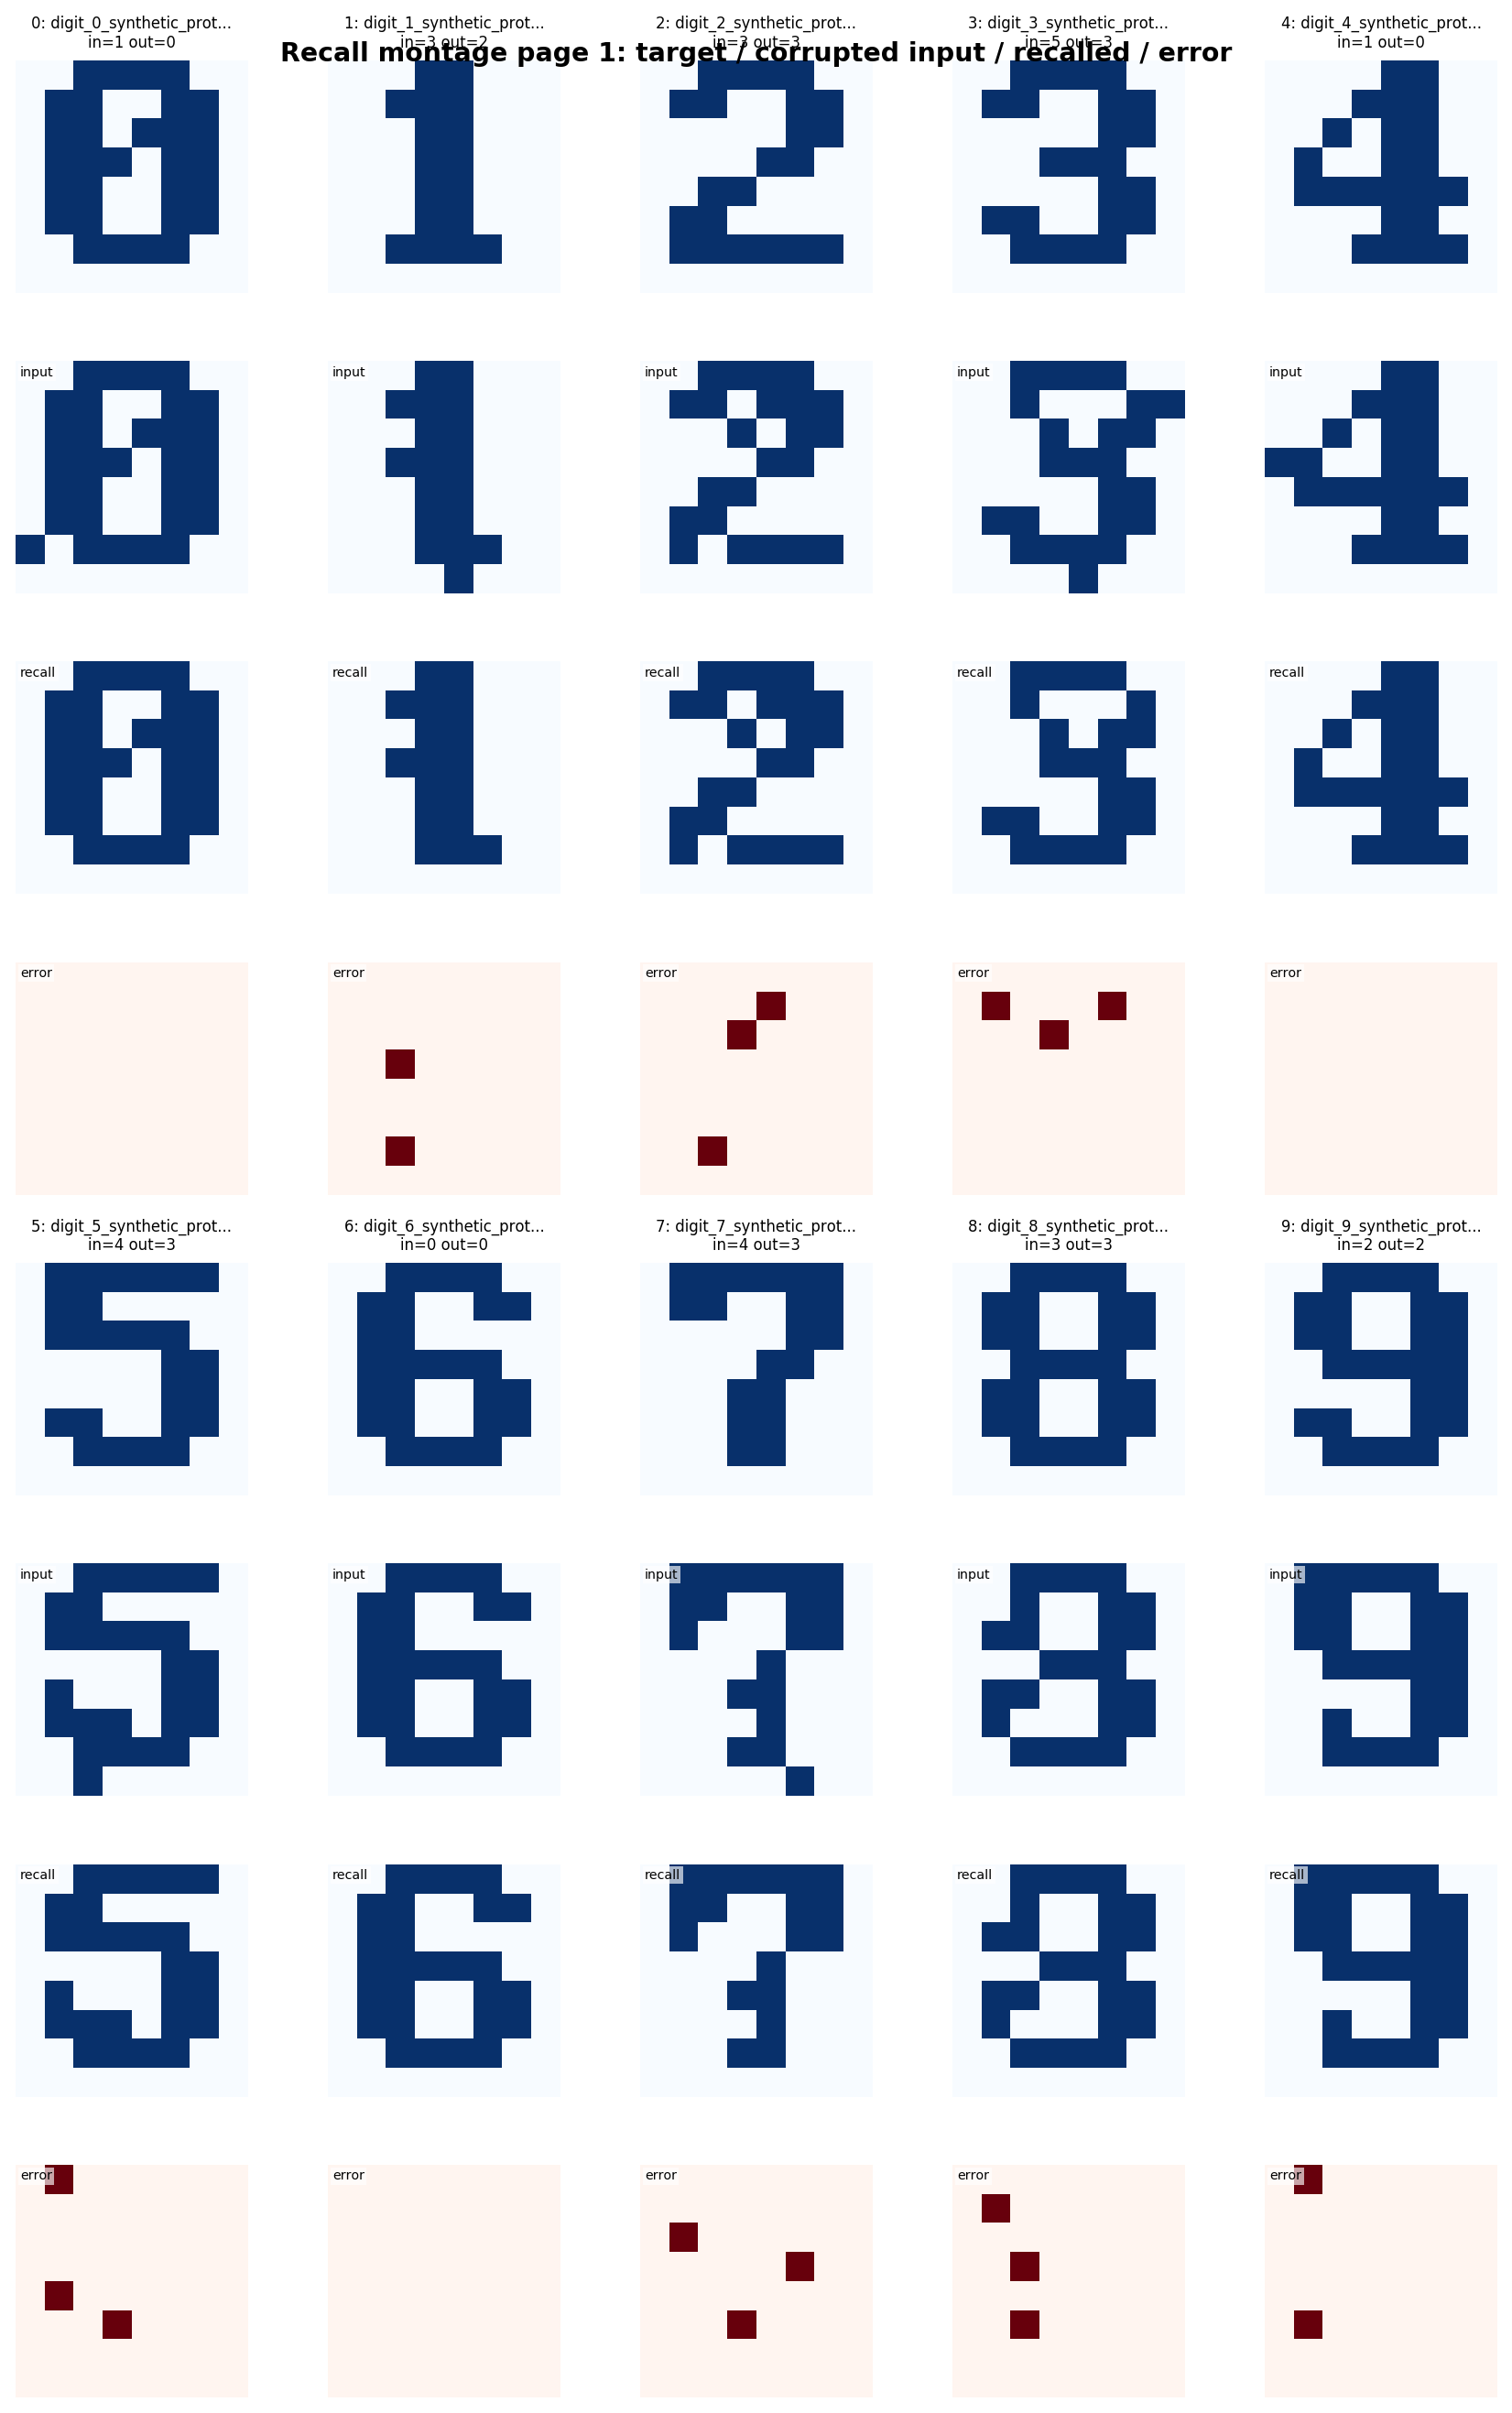
\includegraphics[height=0.76\textheight,keepaspectratio]{output_learning/recall_montage_page_001.png}
  \caption{Recall montage for the ten digit memories. For each digit the
  panels show, from top to bottom, the stored target, the corrupted
  input used to initialise the ODE, the recalled output after relaxation,
  and the pixelwise error image $|\widehat\beta-\beta|$.}
  \label{fig:digit_recall_montage}
\end{figure}

\begin{figure}[htbp]
  \centering
  \begin{minipage}{0.48\linewidth}
    \centering
    
\includegraphics[width=\linewidth]{output_learning/recall_bar.png}
  \end{minipage}
  \hfill
  \begin{minipage}{0.48\linewidth}
    \centering
    
\includegraphics[width=\linewidth]{output_learning/recall_hamming.png}
  \end{minipage}
  \caption{Recall diagnostics. Left: exact-recall fraction for each
  stored digit. Right: input Hamming corruption versus final Hamming
  error. Points below the diagonal indicate denoising by the NDR--FN
  flow.}
  \label{fig:digit_recall_diagnostics}
\end{figure}

\subsection{What the experiment tells us}

The experiment demonstrates the basic mechanism promised by the
preceding sections. A passive resistor mesh can be trained so that a
set of binary image patterns becomes a set of stable fixed points of
the coupled NDR--FN network, and the fixed-point equations are solved
at the level of the physical parameters --- the conductances --- not by
any kind of black-box optimisation. The resulting memories remain stable
under the full nonlinear dynamics.

The recall results also make the limitation concrete. Storing ten digit
prototypes is straightforward for the complete passive mesh with bias:
the fixed-point residuals are tiny and all Jacobians are Hurwitz.
Perfect recall from corrupted images is harder, because it depends on
basin geometry rather than just the existence and stability of the
target equilibria. The natural next step, in the language of neural
ODEs, is trajectory-level training of the flow map: include noisy
versions of each target pattern in the loss, or add hidden nodes,
structured graph templates, or active coupling elements to widen the
basins of attraction.

\begin{thebibliography}{99}

\bibitem{keener2009}
J. Keener and J. Sneyd,
\emph{Mathematical Physiology, Vol.~I: Cellular Physiology},
2nd ed., Springer, New York, 2009.

\bibitem{desoer1969}
C. A. Desoer and E. S. Kuh,
\emph{Basic Circuit Theory},
McGraw-Hill, New York, 1969.

\bibitem{hodgkin1952}
A. L. Hodgkin and A. F. Huxley,
``A quantitative description of membrane current and its application to
conduction and excitation in nerve,''
\emph{Journal of Physiology}, vol.~117, no.~4, pp.~500--544, 1952.

\bibitem{dayan2001}
P. Dayan and L. F. Abbott,
\emph{Theoretical Neuroscience},
MIT Press, Cambridge, MA, 2001.

\bibitem{fitzhugh1961}
R. FitzHugh,
``Impulses and physiological states in theoretical models of nerve membrane,''
\emph{Biophysical Journal}, vol.~1, no.~6, pp.~445--466, 1961.

\bibitem{nagumo1962}
J. Nagumo, S. Arimoto, and S. Yoshizawa,
``An active pulse transmission line simulating nerve axon,''
\emph{Proceedings of the IRE}, vol.~50, no.~10, pp.~2061--2070, 1962.

\bibitem{pei2025}
Y. Pei et al.,
``Ultra robust negative differential resistance memristor for hardware
neuron circuit implementation,''
\emph{Nature Communications}, vol.~16, article 48, 2025.
\href{https://doi.org/10.1038/s41467-024-55293-9}{doi:10.1038/s41467-024-55293-9}

\bibitem{izhikevich2007}
E. M. Izhikevich,
\emph{Dynamical Systems in Neuroscience},
MIT Press, Cambridge, MA, 2007.

\bibitem{strukov2008}
D. B. Strukov, G. S. Snider, D. R. Stewart, and R. S. Williams,
``The missing memristor found,''
\emph{Nature}, vol.~453, pp.~80--83, 2008.

\bibitem{hirsch2013}
M. W. Hirsch, S. Smale, and R. L. Devaney,
\emph{Differential Equations, Dynamical Systems, and an Introduction to Chaos},
3rd ed., Academic Press, Waltham, MA, 2013.

\bibitem{wiggins2003}
S. Wiggins,
\emph{Introduction to Applied Nonlinear Dynamical Systems and Chaos},
2nd ed., Springer, New York, 2003.

\bibitem{khalil2002}
H. K. Khalil,
\emph{Nonlinear Systems},
3rd ed., Prentice Hall, Upper Saddle River, NJ, 2002.

\bibitem{rudin1976}
W. Rudin,
\emph{Principles of Mathematical Analysis},
3rd ed., McGraw-Hill, New York, 1976.

\bibitem{lang1993}
S. Lang,
\emph{Real and Functional Analysis},
3rd ed., Springer, New York, 1993.

\bibitem{horn2013}
R. A. Horn and C. R. Johnson,
\emph{Matrix Analysis},
2nd ed., Cambridge University Press, Cambridge, 2013.

\bibitem{doyle1984}
P. G. Doyle and J. L. Snell,
\emph{Random Walks and Electric Networks},
Mathematical Association of America, Washington, DC, 1984.

\bibitem{bollobas1998}
B. Bollob\'as,
\emph{Modern Graph Theory},
Springer, New York, 1998.

\bibitem{chung1997}
F. R. K. Chung,
\emph{Spectral Graph Theory},
American Mathematical Society, Providence, RI, 1997.

\bibitem{olfati2007}
R. Olfati-Saber, J. A. Fax, and R. M. Murray,
``Consensus and cooperation in networked multi-agent systems,''
\emph{Proceedings of the IEEE}, vol.~95, no.~1, pp.~215--233, 2007.

\bibitem{wu2007}
C. W. Wu,
\emph{Synchronization in Complex Networks of Nonlinear Dynamical Systems},
World Scientific, Singapore, 2007.

\bibitem{chen2018neuralode}
R. T. Q. Chen, Y. Rubanova, J. Bettencourt, and D. Duvenaud,
``Neural ordinary differential equations,''
\emph{Advances in Neural Information Processing Systems}, vol.~31, 2018.

\bibitem{hopfield1982}
J. J. Hopfield,
``Neural networks and physical systems with emergent collective computational abilities,''
\emph{Proceedings of the National Academy of Sciences},
vol.~79, no.~8, pp.~2554--2558, 1982.

\bibitem{amit1985}
D. J. Amit, H. Gutfreund, and H. Sompolinsky,
``Spin-glass models of neural networks,''
\emph{Physical Review A}, vol.~32, no.~2, pp.~1007--1018, 1985.

\end{thebibliography}

\end{document}
